\section{Experimental Results}
The controller's performance was evaluated by tracking a square wave reference signal with a half-period of 5 seconds. The system's response, as shown in Figure~\ref{fig::response}, aligns with the reference system design. The system was able to track the reference signal without significant transient tracking errors (Figure~\ref{fig::error_inputs}) due to input saturation. The steady-state error remained within the bounds of the RPM sensor's resolution (\cite{seshaIdent}).

The high-frequency oscillations in the tracking response are primarily
attributed to the RPM sensors resolution $(\approx 50 \, rad/s)$ and the
switching in robust control input to compensate for the resulting tracking
error. This can be further smoothed by increasing the value of $\varepsilon$,
although this may result in poorer transient performance. The estimated
parameters converged to the actual values (Figure~\ref{fig::param_est}). The
rate of convergence can be further t improved by tuning the adaptation rate
matrix with appropriate scaling based on the ranges of individual parameters.

\begin{figure}[H]
    \centering
    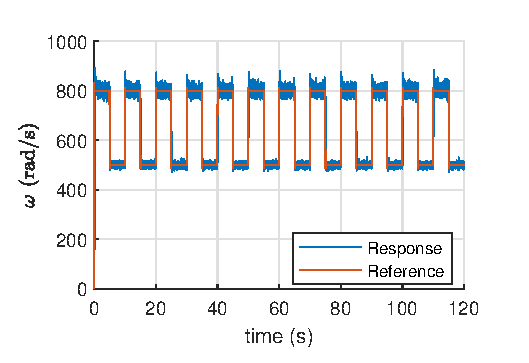
\includegraphics[width = 0.49\textwidth]{Part2/figs/4_figs/results/response.eps}
    \caption{Controller response to a square wave reference signal}
    \label{fig::response}
\end{figure}

\begin{figure}[H]
    \begin{minipage}{0.49\textwidth}
        \begin{figure}[H]
            \centering
            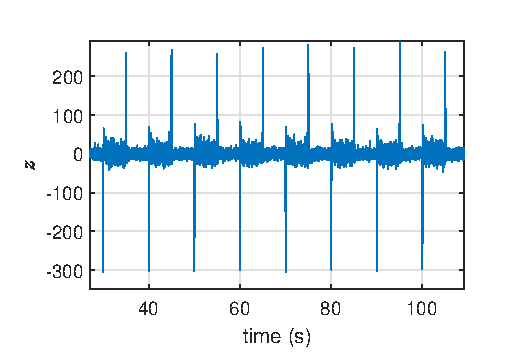
\includegraphics[width=\textwidth]{Part2/figs/4_figs/results/z.eps}
        \end{figure}
    \end{minipage}
    \begin{minipage}{0.49\textwidth}
        \begin{figure}[H]
            \centering
            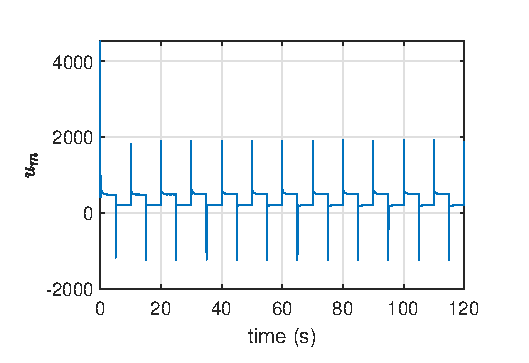
\includegraphics[width=\textwidth]{Part2/figs/4_figs/results/um.eps}
        \end{figure}
    \end{minipage}
\end{figure}
\begin{figure}[H]
    \begin{minipage}{0.49\textwidth}
        \begin{figure}[H]
            \centering
            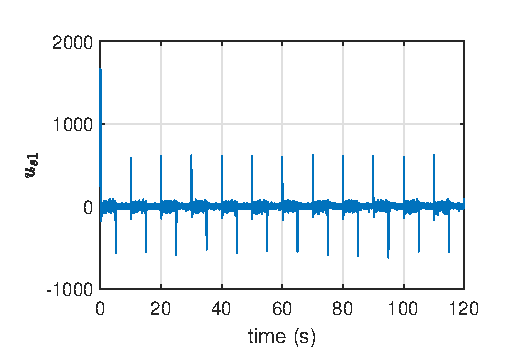
\includegraphics[width=\textwidth]{Part2/figs/4_figs/results/us1.eps}
        \end{figure}
    \end{minipage}
    \begin{minipage}{0.49\textwidth}
        \begin{figure}[H]
            \centering
            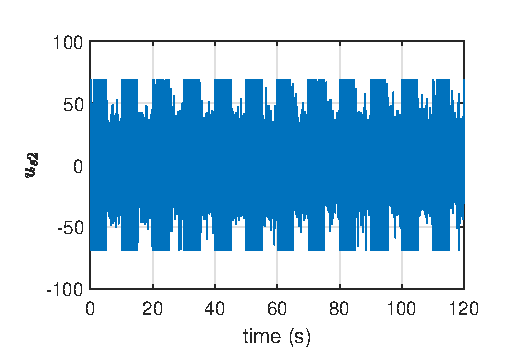
\includegraphics[width=\textwidth]{Part2/figs/4_figs/results/us2.eps}
        \end{figure}
    \end{minipage}
    \caption{Tracking error and control inputs}
    \label{fig::error_inputs}
\end{figure}


\begin{figure}[H]
    \begin{minipage}{0.49\textwidth}
        \begin{figure}[H]
            \centering
            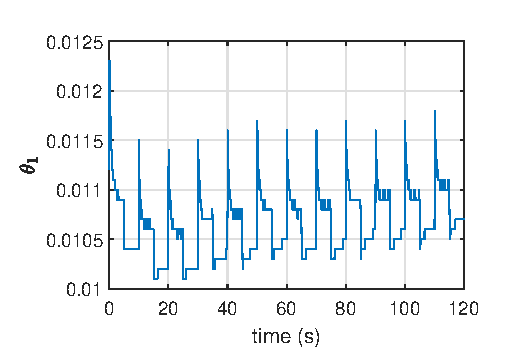
\includegraphics[width=\textwidth]{Part2/figs/4_figs/results/th1.eps}
        \end{figure}
    \end{minipage}
    \begin{minipage}{0.49\textwidth}
        \begin{figure}[H]
            \centering
            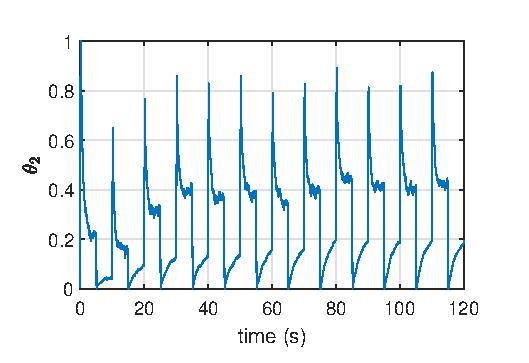
\includegraphics[width=\textwidth]{Part2/figs/4_figs/results/th2.eps}
        \end{figure}
    \end{minipage}
\end{figure}
\begin{figure}[H]
    \begin{minipage}{0.49\textwidth}
        \begin{figure}[H]
            \centering
            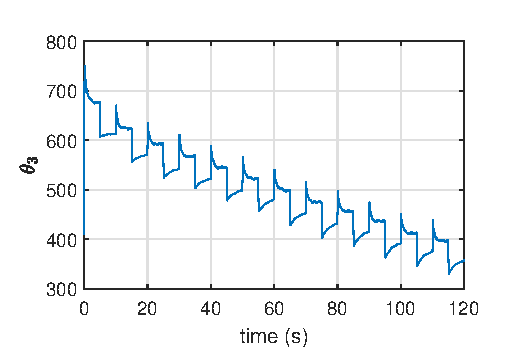
\includegraphics[width=\textwidth]{Part2/figs/4_figs/results/th3.eps}
        \end{figure}
    \end{minipage}
    \begin{minipage}{0.49\textwidth}
        \begin{figure}[H]
            \centering
            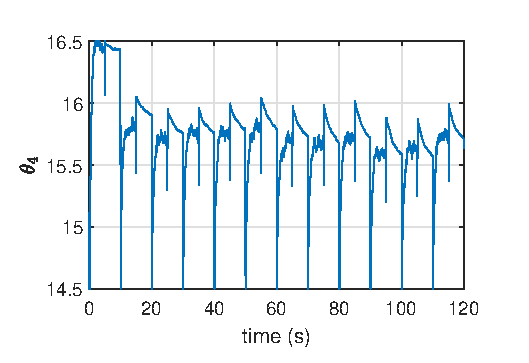
\includegraphics[width=\textwidth]{Part2/figs/4_figs/results/th4.eps}
        \end{figure}
    \end{minipage}
    \caption{Parameter estimation results}
    \label{fig::param_est}
\end{figure}
